\documentclass[12pt,a4paper]{report}
\usepackage[top=1cm, bottom=1.5cm, left=1cm, right=1cm]{geometry}
\usepackage{amsmath,amsfonts,amssymb,mathrsfs,tikz}
\usepackage{eso-pic}
\usepackage{fancyhdr}
\usepackage{multicol}
\setlength{\columnsep}{1cm}
\usepackage[most]{tcolorbox}
\newcommand{\N}{\mathbb{N}}
\usetikzlibrary[patterns]
\usetikzlibrary{shapes.geometric}
\usetikzlibrary{decorations.pathmorphing}
\tcbuselibrary{skins}
%\usetikzlibrary{shapes.geometric}
\pagestyle{fancy}
\renewcommand{\headrulewidth}{0pt}
\cfoot{\thepage}
\renewcommand{\labelenumi}{%
	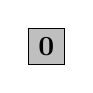
\begin{tikzpicture}[baseline=(1.base)]
	\node[draw,regular polygon,regular polygon sides=4,inner sep=.5mm,fill=gray!50,font=\bfseries](1){\arabic{enumi}};
	\end{tikzpicture}}
\renewcommand{\labelenumii}{%
	
\begin{tikzpicture}[baseline=(1.base)]
	\node[draw,circle,inner sep=.5mm,fill=gray!15,font=\bfseries\footnotesize,minimum size=5mm](1){\alph{enumii}};
	\end{tikzpicture}}

	\usepackage[object=vectorian]{pgfornament}
%\newcolumntype{X}{p{0.3\linewidth}}
\newtcolorbox[auto counter]{exo}{breakable,enhanced,before skip=5mm,after skip=5mm,title={Exercice \thetcbcounter},attach boxed title to top left={yshift=-3mm},boxsep=3mm,boxrule=2pt,colframe=black,colback=white,coltitle=black}
\parindent=0mm
\pagestyle{fancy}

	\fancyfoot[R]{Pr: S.BASSY}
	\fancyfoot[L]{bassy.soufiane@gmail.com}
\newcommand{\R}{\mathbb{R}}
\begin{document}

\begin{tcolorbox}[colback=gray!5]
	
	
	\begin{center}
		\begin{tabular}{c c  c}
			2020/2021 	\hspace*{3cm}   & \textbf{{\huge Devoir   $1$  }} & 	\hspace*{3cm} Classes:.............			\\
			Pr: S.BASSY\hspace*{3cm} &{\large Durée:$2$h} & \hspace*{3cm}Lycée: ..............
		\end{tabular}
	\end{center}
\end{tcolorbox}


\begin{exo}
	\begin{enumerate}
\item QSt\hfill 1pt
\item QSt\hfill 1pt
\item QSt\hfill 1pt
\item QSt\hfill 1pt
\end{enumerate}
\end{exo}
%%%%%%%%%%%%%%%%%%%%%%%%%%%%% exercice 2
\begin{exo}
		\begin{enumerate}
		\item 
		
		\begin{enumerate}
			\item  QSt        \hfill 1pt
			\item QSt        \hfill 1pt
			\item QSt        \hfill 1pt
			\item QSt         \hfill 1pt
		\end{enumerate}
		\item QSt\hfill 1pt
		\item QSt\hfill 1pt
		\item QSt\hfill 1pt
	\end{enumerate}
\end{exo}



\begin{exo}
	\begin{enumerate}
		\item QSt\hfill 1pt
		\item QSt\hfill 1pt
		\item QSt\hfill 1pt
		\item QSt\hfill 1pt
	\end{enumerate}
\end{exo}

\begin{exo}
	\begin{enumerate}
		\item 
		
		\begin{enumerate}
			\item  QSt        \hfill 1pt
			\item QSt        \hfill 1pt
			\item QSt        \hfill 1pt
			\item QSt         \hfill 1pt
		\end{enumerate}
		\item QSt\hfill 1pt
		\item QSt\hfill 1pt
		\item QSt\hfill 1pt
		\item QSt\hfill 1pt
		\item QSt\hfill 1pt
		\item QSt\hfill 1pt
	\end{enumerate}
\end{exo}
	\begin{center}
	\pgfornament[color=black,width=2cm]{33} \Large{Bonne chance } \pgfornament[color=black,width=2cm]{34}

\end{center}


%%%%%%%%%%%%%%%%%%%%%%%%%%%%%%%%%%%




\end{document}